%%%%%%%%%%%%%%%%%%%%%%%%%%%%%%%%%%%%%%%%%%%%%%%%%%%%%%%%%%%%%%%%%%%%%%%%%%%%%%%%
\chapter{Постановка задачи и выбор пути решения}
%%%%%%%%%%%%%%%%%%%%%%%%%%%%%%%%%%%%%%%%%%%%%%%%%%%%%%%%%%%%%%%%%%%%%%%%%%%%%%%%

В данном разделе перечислены задачи, решаемые в ходе работы над данной магистерской диссертацией. Также в данном разделе указаны требования и ограничения, стоящие при выполнении поставленных задач.

%%%%%%%%%%%%%%%%%%%%%%%%%%%%%%%%%%%%%%%%%%%%%%%%%%%%%%%%%%%%%%%%%%%%%%%%%%%%%%%%
\section{Решаемые задачи}
%%%%%%%%%%%%%%%%%%%%%%%%%%%%%%%%%%%%%%%%%%%%%%%%%%%%%%%%%%%%%%%%%%%%%%%%%%%%%%%%

Ниже перечислены поставленные для данной магистерской диссертации задачи:
%
\begin{itemize*}
\item Разработать метод извлечения структуры спецификации, формирования сигнатур функций, типов данных, автоматов и др.;
\item Разработать метод извлечения аннотаций, которые описывают влияние функции на окружающую среду;
\item Убедиться в правильности сгенерированной формальной спецификации на языке LibSL
\end{itemize*}
%

%%%%%%%%%%%%%%%%%%%%%%%%%%%%%%%%%%%%%%%%%%%%%%%%%%%%%%%%%%%%%%%%%%%%%%%%%%%%%%%%
\section{Формулирование требований к разрабатываемой системе}
%%%%%%%%%%%%%%%%%%%%%%%%%%%%%%%%%%%%%%%%%%%%%%%%%%%%%%%%%%%%%%%%%%%%%%%%%%%%%%%%

%%%%%%%%%%%%%%%%%%%%%%%%%%%%%%%%%%%%%%%%
\subsection{Требования к методу извлечения структуры спецификации}
%%%%%%%%%%%%%%%%%%%%%%%%%%%%%%%%%%%%%%%%

Метод извлечения структуры спецификации и формирования сигнатур функций, типов данных и автоматов, должен быть рассчитан на использование с языком Java.

Метод должен корректно обрабатывать код на языке Java 8.

Метод должен иметь возможность работать как с исходным кодом(java-файлами) библиотеки, так и с jar-файлом библиотеки.

В процессе извлечения структуры спецификации не должен извлекать исходный код функций. Процесс касается лишь сигнатур функций, типов данных, автоматов и др.

Метод извлечения структуры спецификации должен исключать все интерфейсы, которые присутствуют в библиотеке, а также те классы, которые не относятся к библиотеке.
Также необходимо исключать из анализа абстрактные классы и методы из библиотеки.

Метод извлечения структуры спецификации должен обрабатывать все основные элементы программы, в которых используется библиотека: возвращаемое методом значение, аргументы метода, типы методов.

Метод извлечения структуры спецификации должен в процессе работы формировать объекты , которые являются элементами LibSL спецификации:
%
\begin{itemize*}
\item Описание псевдонимов типов
\item Описание классов автоматов
\item Описание функций API библиотеки
\end{itemize*}
%

Полученный код инструментом должен быть удобочитаемым для программиста. Например, имена переменных из сигнатуре функции библиотеки должны сохраняться, если это возможно.

%%%%%%%%%%%%%%%%%%%%%%%%%%%%%%%%%%%%%%%%
\subsection{Требования к методу извлечения аннотаций}
%%%%%%%%%%%%%%%%%%%%%%%%%%%%%%%%%%%%%%%%

Разрабатываемой метод должен дополнять структуру спецификации, метод формирования которой описан выше.

Разрабатываемый инструмент должен быть кроссплатформенным и работать под управлением операционных систем

Метод извлечения аннотаций не должен ухудшать сформировнную структуру формальной спецификации библиотеки.

Информация полученая методом извлечения аннотаций должна записываться в определенную аннотацию в языке LibSL.

%%%%%%%%%%%%%%%%%%%%%%%%%%%%%%%%%%%%%%%%
\subsection{Ограничения разрабатываемого инструмента генерации формальной спецификации}
%%%%%%%%%%%%%%%%%%%%%%%%%%%%%%%%%%%%%%%%

Метод извлечения аннотаций должен решать проблему только извлечения информации о влиянии функции на окружающую среду.
То есть, при анализе исходного кода все аргументы метода, которые каким-либо образом изменяются в функции (например, поле объекта одного из аргументов функции асайнится в теле метода на другое значение), будут выделены в отдельную аннотацию в языке LibSL.
Решение проблемы извлечения контрактов (предусловий, постусловий и инвариантов) функции,
остаются за рамками выполнения данной работы, так как выделенные две проблемы являются очень сложными задачами,
поэтому в работе был сделан упор на извлечения аннотаций, которые описывают влияние функции на окружающую среду.

Проблема извлечения окружения состояния автоматов и переходов автоматов по той же причине остается за рамками этой работы.

%%%%%%%%%%%%%%%%%%%%%%%%%%%%%%%%%%%%%%%%%%%%%%%%%%%%%%%%%%%%%%%%%%%%%%%%%%%%%%%%
\section{Анализ задач и выбор пути решения}
%%%%%%%%%%%%%%%%%%%%%%%%%%%%%%%%%%%%%%%%%%%%%%%%%%%%%%%%%%%%%%%%%%%%%%%%%%%%%%%%

Далее будет рассмотрен существующий вид статического анализа - анализ потока управления.
Ниже перечислены основные методы, которые можно выделить из такого вида статического анализа исходного кода или байт-кода библиотеки:
%
\begin{itemize*}
\item Метод анализа графа потока управления (CFG);
\item Метод анализа абстрактного синтаксического дерева (AST);
\end{itemize*}
%
\nomenclature{AST}{Abstract Syntax Tree}
\nomenclature{CFG}{Control Flow Graph}

Суть методов заключается в построение графа потока управления, который на входе получает исходный код программы и представляет его в виде удобной модели программы для проведения анализа потока данных.
Модели программы обеспечивают доступ ко всем объектам программного кода и их атрибутам. Также поддерживают эффективный поиск объектов и снимают сложность разработки методов статического анализа.

%%%%%%%%%%%%%%%%%%%%%%%%%%%%%%%%%%%%%%%%
\subsection{Метод анализа графа потока управления}
%%%%%%%%%%%%%%%%%%%%%%%%%%%%%%%%%%%%%%%%

Граф потока управления представляется в виде ориентированного графа. В нем сохраняется вся необходимая информация о конструкциях программы и переходах между ними.

При построение CFG также учитываются:
%
\begin{itemize*}
\item Безусловные переходы;
\item Ветвления;
\item Циклы;
\item Вызовы функций;
\item Исключения;
\end{itemize*}
%

\begin{figure}[htbp]
\centering
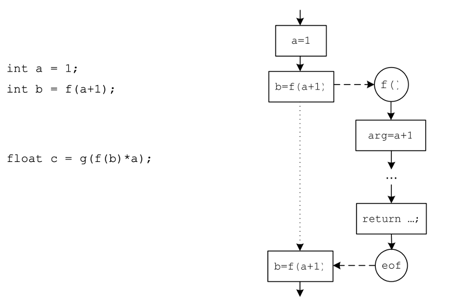
\includegraphics[width=\textwidth]{fig/cfg_example_1.png}
\caption{Пример CFG}%
\label{fig:cfg_example_1}
\end{figure}

%%%%%%%%%%%%%%%%%%%%%%%%%%%%%%%%%%%%%%%%
\subsection{Метод анализа абстрактного синтаксического дерева}
%%%%%%%%%%%%%%%%%%%%%%%%%%%%%%%%%%%%%%%%

Абстрактное синтаксическое дерево представляет собой древовидное представление структуры исходного кода, где листья представляются в качестве константы или переменной, а внутренние узлы - операторы.

\begin{figure}[htbp]
\centering
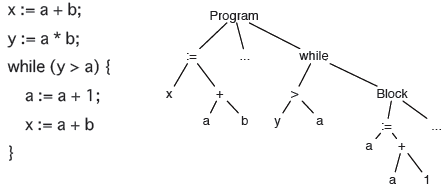
\includegraphics[width=\textwidth]{fig/ast_example_1.png}
\caption{Пример AST}%
\label{fig:ast_example_1}
\end{figure}

AST используют как в разработке программ, так и в анализе программ.
AST лучше всего представляет синтаксическую структуру исходного кода. AST независим от конкретного синтаксиса для идентификаторов, операторов, условий или утверждений базового языка программирования.

Представление AST можно считать не только промежуточным, а также использовать его для различных оптимизаций. Преимуществом использования абстрактного синтаксического дерева является более высокий уровень абстракции по сравнению с исходным кодом программы.

Как писалось ранее, существую подходы, позволяющие построить модель исходного кода в виде диаграмм UML. Но, по моему мнению, AST подходит лучше для представления информации о выполнении программы.

В данной работе AST используется в методе извлечения аннотаций, которые описывают влияние функции на окружающую среду.

%%%%%%%%%%%%%%%%%%%%%%%%%%%%%%%%%%%%%%%%%%%%%%%%%%%%%%%%%%%%%%%%%%%%%%%%%%%%%%%%
\section{Выводы}
%%%%%%%%%%%%%%%%%%%%%%%%%%%%%%%%%%%%%%%%%%%%%%%%%%%%%%%%%%%%%%%%%%%%%%%%%%%%%%%%

В данном разделе были сформулированы задачи, которые актуальны для этой магистерской работы. Были определены требования и ограничения к разрабатываемой системе автоматизации генерации формальной спецификации библиотек.
В ходе анализа задачи было принято решение об использовании статического анализа кода, а именно метода анализа абстрактного синтаксического дерева при проектировании метода извлечения аннотаций.